\chapter{Gedragsecologie}\label{ch:b3:behavioural-ecology}

Een stokstaartje staat op een termietenheuvel terwijl de rest van de
groep naar voedsel graaft, en wanneer er een havik verschijnt blaft het
en schieten de anderen hun holen in. De schildwacht heeft een uur lang
niet gegeten en heeft zichzelf tot het meest opvallende dier van de
woestijn gemaakt. Waarom? Een pauw sleept een staart mee die hem een
vijfde van zijn energiebudget kost en zijn vlucht voor tijgers
vertraagt. Een honingbij die van een veld terugkeert danst op een
verticale raat, en de hoek van haar dans met de verticaal is de hoek van
het voedsel met de zon. Een koolmees die rupsen zoekt in een plukje
gebladerte verlaat het terwijl er nog rupsen te vinden zijn. Geen van
deze dieren heeft dit hoofdstuk gelezen, en toch gedraagt elk zich
alsof het een optimalisatie, een spel of een probleem in
verwantschapsboekhouding had opgelost. De gedragsecologie bestudeert
gedrag als een stel geëvolueerde oplossingen: waar een gedrag voor
dient, in termen van de genen die het verspreidt, en wat zijn kosten en
baten moeten zijn opdat de natuurlijke selectie het heeft
voortgebracht. Haar gereedschap is dat van een econoom ---
optimalisatie, speltheorie, de boekhouding van de verwantschap --- en
haar toetssteen is het veld.

\section{Vier vragen en de machinerie van het instinct}

\begin{definition}[De vragen van Tinbergen]\label{def:b3:behavioural-ecology:tinbergen}
\index{vier vragen van Tinbergen}\index{vast handelingspatroon}\index{sleutelprikkel}\index{inprenting}\index{kritieke periode}
Tinbergen (1963) zei dat een volledige verklaring van welk gedrag dan
ook vier vragen moet beantwoorden: zijn \emph{mechanisme} (welke
prikkels en welke neurale machinerie het voortbrengen), zijn
\emph{ontwikkeling} (hoe het in het individu ontstaat, uit genen en
ervaring), zijn \emph{functie} (hoe het aan overleving en voortplanting
bijdraagt) en zijn \emph{evolutionaire geschiedenis} (hoe het uit
voorouderlijk gedrag is ontstaan). De ethologen die ze formuleerden
hadden de eerste twee vastgelegd. Veel gedragingen zijn \emph{vaste
handelingspatronen}: gestandaardiseerde reeksen die door een eenvoudige
\emph{sleutelprikkel} worden vrijgemaakt en, eenmaal begonnen, tot het
einde worden uitgevoerd --- een grauwe gans rolt een verschoven ei met
haar snavel naar het nest terug, en maakt de beweging af ook als het ei
halverwege wordt weggenomen; een kuiken van een zilvermeeuw pikt naar
een rode vlek op elk snavelvormig voorwerp, en pikt vaker naar een
stokje met drie rode banden dan naar de kop van een echte meeuw; een
mannetje van de stekelbaars valt alles aan wat rood is aan de
onderkant, ook een voorbijrijdende postwagen die het door het raam
ziet. Andere worden binnen een venster geleerd: de \emph{inprenting},
waardoor een gansje op zijn eerste dag volgt en daarna als ouder
behandelt wat er ook beweegt --- een gans, Lorenz, een kartonnen doos
--- is snel, onomkeerbaar en beperkt tot een \emph{kritieke periode};
het leren van zang bij vogels, het voorbeeld uit het deel van het
tweede jaar, heeft dezelfde vorm. De tweedeling tussen aangeboren en
geleerd is onjuist: een gedrag heeft een genetisch programma dat
vastlegt wat er moet worden geleerd, wanneer en van wie, en dat
programma is wat evolueert.
\end{definition}

\begin{proof}[Bewijsmateriaal]
De veldexperimenten van Tinbergen legden de methode vast. Bijenwolven
(\emph{Philanthus}) keren terug naar een nest dat in het zand verborgen
ligt; hij verplaatste een ring dennenappels die hij rond één ingang had
gelegd terwijl de wesp weg was, en zij zocht in het midden van de
verplaatste ring --- zij had de herkenningspunten geleerd. Kokmeeuwen
halen na het uitkomen de eierschalen uit het nest; hij legde eieren
naast beschilderde schalen, natuurlijke schalen en andere voorwerpen,
en telde welke de kraaien meenamen: het witte binnenvlak van een schaal
trok roofdieren aan, en het opruimen dat op netheid had geleken was
camouflage. De proeven met meeuwenkuikens maakten een \omterm{def:b3:behavioural-ecology:tinbergen}{sleutelprikkel}
meetbaar door kartonnen koppen aan te bieden die telkens op één kenmerk
varieerden. De ingeprente ganzen van Lorenz volgden hem levenslang;
eenden die op hun eerste dag op een bewegende doos waren ingeprent
waren daarna niet meer zover te krijgen dat zij een eend volgden.
\end{proof}

\begin{omfigure}
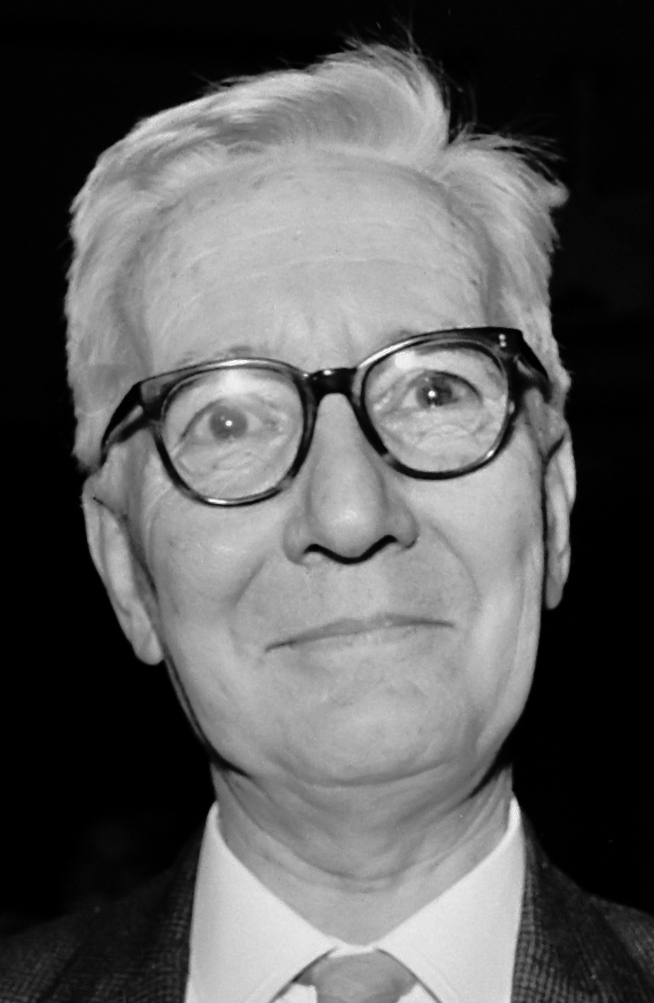
\includegraphics[width=0.36\linewidth]{images/book5/tinbergen.jpg}\hspace{0.04\linewidth}
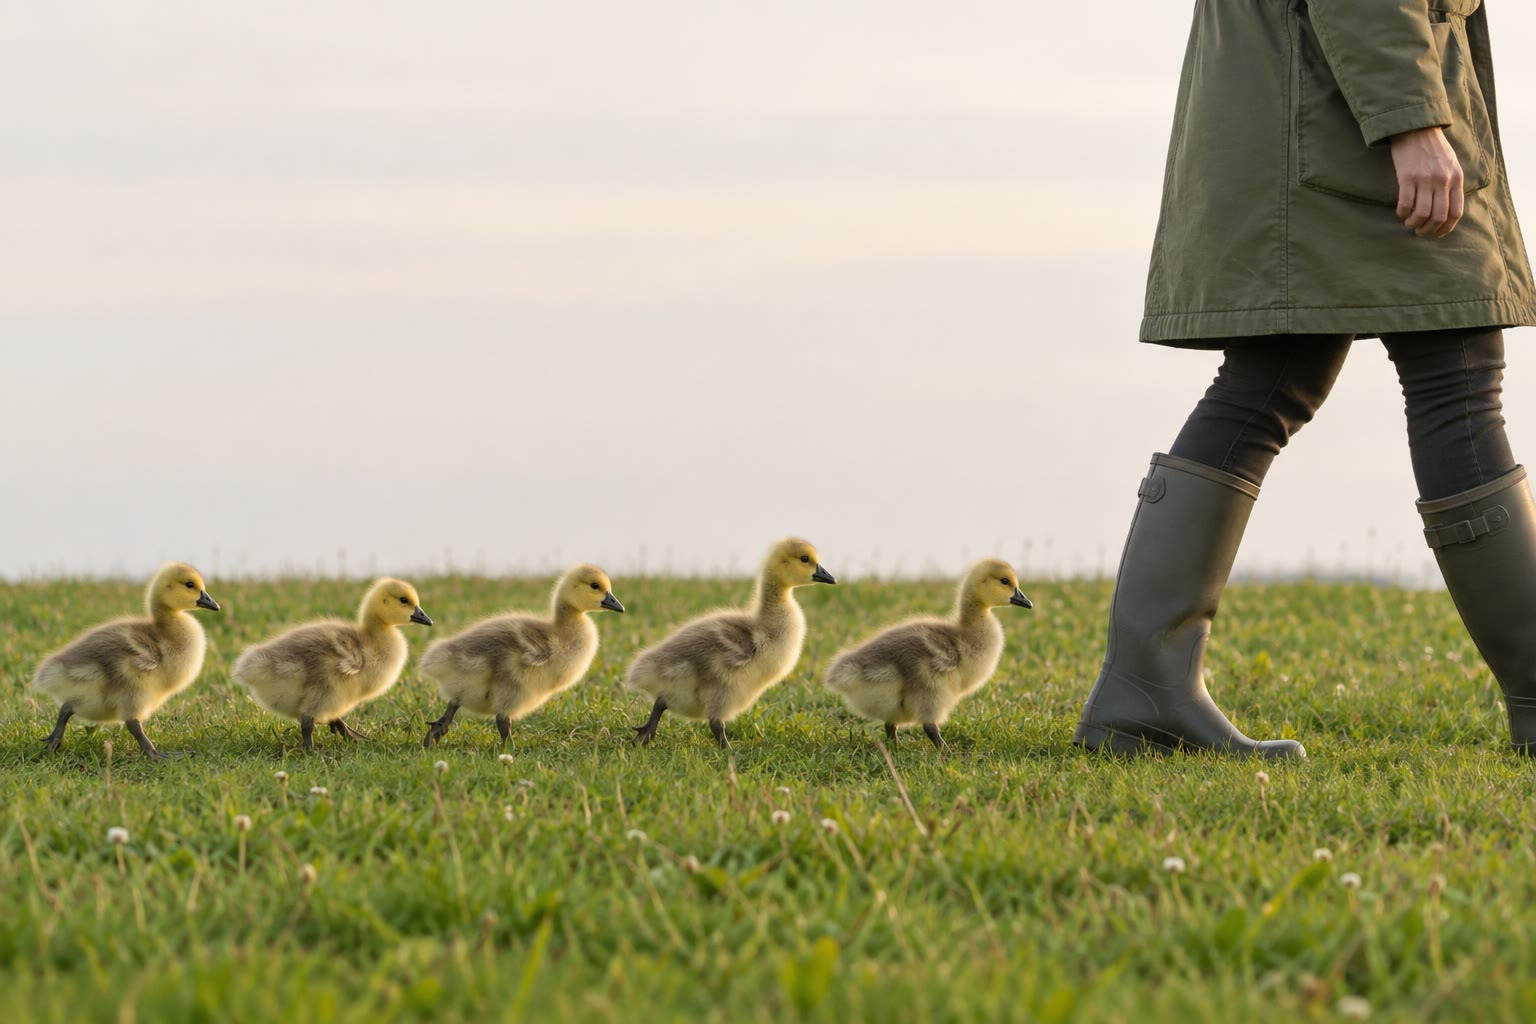
\includegraphics[width=0.52\linewidth]{images/book5/ai/b5-26-goose-imprinting.jpg}

{\small Links: Niko Tinbergen (1907--1988), die de vragen van het gedrag
mee het veld in nam en er experimenten van maakte (foto door Rob
Mieremet, Anefo, 1973, CC0). Rechts: gansjes die het eerste grote
bewegende ding volgen dat zij zagen, een dag na het uitkomen, en die
daarna nooit meer van gedachten zijn te doen veranderen.}
\end{omfigure}

\section{Beslissen: optimaal foerageren}

\begin{theorem}[De stelling van de marginale waarde]\label{thm:b3:behavioural-ecology:mvt}
\index{optimaal foerageren}\index{stelling van de marginale waarde}\index{verblijftijd in een plek}\index{valuta}
Een foerageerder bezoekt plekken met voedsel die door een reistijd
$\tau$ van elkaar zijn gescheiden. In een plek wint hij een energie
$g(t)$ na tijd $t$, met $g$ stijgend en concaaf (de plek raakt
uitgeput). Verlaat hij elke plek na tijd $t$, dan is zijn tempo van
winst op den duur $R(t) = g(t)/(\tau + t)$, en voldoet de verblijftijd
$t^{*}$ die dat maximaliseert aan
\[
g'(t^{*}) = \frac{g(t^{*})}{\tau + t^{*}} = R(t^{*}) :
\]
verlaat een plek wanneer het ogenblikkelijke tempo van winst erin is
gedaald tot het gemiddelde tempo over het hele leefgebied, de reis
inbegrepen (Charnov, 1976). Gevolgen: hoe langer de reistijd, hoe
langer het verblijf en hoe grondiger elke plek wordt uitgeput; in een
rijker leefgebied (een hogere $R$) wordt elke plek eerder en minder
uitgeput verlaten; en alle plekken worden bij hetzelfde marginale tempo
verlaten wat hun kwaliteit ook is, zodat een arme plek vrijwel meteen
wordt verlaten en een rijke pas wanneer zij tot het gemiddelde van het
leefgebied is afgewerkt. Voor $g(t) = A(1 -
\mathrm{e}^{-t/T_{0}})$ wordt de voorwaarde $(\tau + t^{*})/T_{0} =
\mathrm{e}^{t^{*}/T_{0}} - 1$, numeriek op te lossen: met $\tau = T_{0}$
is $t^{*} \approx 1.15\,T_{0}$; met $\tau = 4T_{0}$ is $t^{*} \approx
2.0\,T_{0}$.
\end{theorem}
\begin{proof}
$R(t) = g(t)/(\tau + t)$; $R'(t) = [g'(t)(\tau + t) - g(t)]/(\tau +
t)^{2} = 0$ geeft $g'(t^{*}) = g(t^{*})/(\tau + t^{*})$. Meetkundig:
teken $g$ tegen $t$ met de oorsprong in $-\tau$; $R(t)$ is de helling
van de lijn van $(-\tau, 0)$ naar $(t, g(t))$, maximaal waar die lijn
aan de kromme raakt --- en dat is de voorwaarde. Een grotere $\tau$
verschuift de oorsprong naar links en het raakpunt naar rechts; een
rijker leefgebied maakt de raaklijn steiler en verplaatst haar naar
links. Voor de e-macht is $g' = (A/T_{0})
\mathrm{e}^{-t/T_{0}}$ en $g/(\tau + t) = A(1 - \mathrm{e}^{-t/T_{0}})/
(\tau + t)$; gelijkstellen en herschikken geeft de genoemde
vergelijking, en invullen van $t^{*} = 1.15T_{0}$ met $\tau = T_{0}$:
links $2.15$, rechts $\mathrm{e}^{1.15} - 1 = 2.16$.
\end{proof}

\begin{omfigure}
\begin{tikzpicture}
\begin{axis}[
  width=0.68\linewidth, height=5.8cm,
  axis x line=middle, axis y line=left,
  xmin=-4.5, xmax=5, ymin=0, ymax=1.15,
  xlabel={tijd (in eenheden $T_{0}$)}, ylabel={energie gewonnen in de plek},
  xlabel style={font=\small, at={(axis description cs:0.95,0.0)}, anchor=north}, ylabel style={font=\small},
  tick label style={font=\small}, xtick={-4,-1,0,1.15,2}, xticklabels={$-4T_0$,$-T_0$,0,$1.15$,$2.0$}, ytick={0.5,1}, yticklabels={$0.5A$,$A$},
  clip=false,
]
\addplot[very thick, omDef, domain=0:5, samples=80] {1-exp(-x)};
\draw[thick, omThm] (axis cs:-1,0) -- (axis cs:1.55,1.13);
\draw[thick, omMeth!70!black] (axis cs:-4,0) -- (axis cs:3.5,1.081);
\fill[omThm] (axis cs:1.15,0.6834) circle (2pt); \fill[omMeth!70!black] (axis cs:2,0.8647) circle (2pt);
\draw[dashed, gray] (axis cs:1.15,0) -- (axis cs:1.15,0.6834); \draw[dashed, gray] (axis cs:2,0) -- (axis cs:2,0.8647);
\node[font=\scriptsize, omThm, anchor=north west, align=left] at (axis cs:-4.4,1.1) {korte reis, $\tau = T_{0}$:\\vertrek bij $t^{*} = 1.15\,T_{0}$,\\plek \qty{68}{\%} uitgeput};
\node[font=\scriptsize, omMeth!70!black, anchor=north west, align=left] at (axis cs:2.4,0.62) {lange reis, $\tau = 4T_{0}$:\\vertrek bij $t^{*} = 2.0\,T_{0}$,\\\qty{86}{\%} uitgeput};
\node[font=\scriptsize, omDef, anchor=north west] at (axis cs:3.0,0.86) {$g(t) = A(1 - \mathrm{e}^{-t/T_{0}})$};
\node[font=\scriptsize, gray, anchor=south] at (axis cs:-2.5,0.02) {reis};
\end{axis}
\end{tikzpicture}

{\small De \omterm{thm:b3:behavioural-ecology:mvt}{stelling van de marginale waarde} getekend. De winstkromme
vlakt af naarmate de plek uitgeput raakt; de lijn van het begin van de
reis naar een punt op de kromme heeft een helling gelijk aan het
algemene tempo van winst; het beste ogenblik om te vertrekken is waar
die lijn raakt. Een langere reis verschuift de oorsprong naar links en
het raakpunt naar rechts.}
\end{omfigure}

\begin{proof}[Bewijsmateriaal]
Cowie (1977) liet koolmezen in een volière meelwormen zoeken die in
bekers vol zaagsel waren verstopt, waarbij de reistijd tussen de bekers
werd geregeld met deksels die meer of minder tijd kostten om te
verwijderen; de vogels bleven langer in elke beker wanneer de reis
trager was, in overeenstemming met de voorspelling van de stelling, en
schoten daar iets overheen in de richting die het meerekenen van de
energiekosten van het reizen verklaart. Spreeuwen die emelten naar hun
jongen brachten (Kacelnik, 1984) namen grotere vrachten mee van
voederplaatsen die verder weg lagen, opnieuw zoals de oplossing vergt
die het tempo bij een laadkromme maximaliseert. Geen van beide proeven
bewijst dat vogels raaklijnen berekenen; beide laten zien dat de
selectie vuistregels heeft voortgebracht wier uitkomst dicht bij het
optimum ligt.
\end{proof}

\section{Wedstrijden: speltheorie}

\begin{proposition}[Havik--Duif en de evolutionair stabiele strategie]\label{prop:b3:behavioural-ecology:hawk-dove}
\index{speltheorie}\index{spel Havik--Duif}\index{evolutionair stabiele strategie}\index{frequentieafhankelijke selectie}
Wanneer het beste gedrag afhangt van wat anderen doen, is er geen
optimum, alleen een \emph{spel}. Twee dieren betwisten een hulpbron die
$V$ waard is; een \emph{Havik} vecht tot hij gewond raakt (kosten $C$)
of wint, een \emph{Duif} vertoont en trekt zich terug als hij wordt
aangevallen. De gemiddelde opbrengsten zijn
\[
\begin{array}{c|cc}
 & \text{tegen Havik} & \text{tegen Duif}\\ \hline
\text{Havik} & (V - C)/2 & V\\
\text{Duif} & 0 & V/2
\end{array}
\]
Een \emph{\omterm{prop:b3:behavioural-ecology:hawk-dove}{evolutionair stabiele strategie}} (Maynard Smith en Price,
1973) is er een die, eenmaal algemeen, door geen enkel zeldzaam
alternatief kan worden binnengedrongen. Is $V > C$, dan is Havik de
ESS: vechten loont zelfs tegen vechters. Is $V
< C$, dan is geen van beide zuivere strategieën stabiel --- een
populatie Duiven wordt binnengedrongen door Haviken, die elke wedstrijd
winnen, en een populatie Haviken door Duiven, die de verwondingen
vermijden --- en is de ESS om Havik te spelen met kans
\[
p^{*} = \frac{V}{C},
\]
of, wat op hetzelfde neerkomt, een populatie waarin dat deel Havik is.
Bij de ESS doen de twee strategieën het even goed, met elk gemiddeld
$V(1 -
V/C)/2$, minder dan de $V/2$ die een populatie Duiven had gedeeld: de
wedstrijd kost iedereen iets, en niemand kan er in zijn eentje beter
van worden. De selectie is hier \emph{frequentieafhankelijk}: de
fitness van een strategie daalt naarmate zij algemener wordt, en daarom
bestaan wedstrijden bij dieren meestal uit vertoon en af en toe uit
oorlog, en daarom blijft het mengsel bestaan.
\end{proposition}
\begin{proof}
Zij $p$ het deel dat Havik speelt. De verwachte opbrengst van een Havik
is $W_{H} = p(V
- C)/2 + (1 - p)V$; die van een Duif is $W_{D} = (1 - p)V/2$. $W_{H} - W_{D} =
p(V - C)/2 + (1 - p)V/2 = [V - pC]/2$, positief voor $p < V/C$ en
daarboven negatief: Haviken breiden zich uit wanneer zij zeldzaam zijn
en worden uitgedund wanneer zij algemeen zijn, en de frequentie komt
uit waar $W_{H} = W_{D}$, bij $p^{*} = V/C$. Dat dit stabiel is volgt
uit de tekenwissel: een verstoring van $p$ boven $p^{*}$ begunstigt
Duiven en wordt gecorrigeerd, eronder begunstigt zij Haviken. Is $V
\ge C$, dan is het verschil positief voor alle $p \le 1$ en legt Havik
zich vast. De gemeenschappelijke opbrengst bij $p^{*}$: $W_{D} = (1 - V/C)V/2$.
\end{proof}

\begin{omfigure}
\begin{tikzpicture}
\begin{axis}[
  width=0.6\linewidth, height=5.4cm,
  axis x line=bottom, axis y line=left,
  xmin=0, xmax=1, ymin=-1, ymax=4.2,
  xlabel={deel Haviken $p$}, ylabel={verwachte opbrengst},
  xlabel style={font=\small, at={(axis description cs:0.5,-0.12)}, anchor=north}, ylabel style={font=\small},
  tick label style={font=\small}, xtick={0,0.5,1}, xticklabels={0,$p^{*} = V/C$,1}, ytick={0,1,2,4},
  clip=false,
]
\addplot[very thick, omThm, domain=0:1, samples=2] {x*(4-8)/2 + (1-x)*4};
\addplot[very thick, omDef, domain=0:1, samples=2] {(1-x)*4/2};
\draw[dashed, gray] (axis cs:0.5,-1) -- (axis cs:0.5,1);
\fill[black] (axis cs:0.5,1) circle (2pt);
\node[font=\scriptsize, omThm, anchor=north west] at (axis cs:0.5,3.9) {Havik: $p(V - C)/2 + (1 - p)V$};
\node[font=\scriptsize, omDef, anchor=south west] at (axis cs:0.62,0.9) {Duif: $(1 - p)V/2$};
\node[font=\scriptsize, anchor=west, align=left] at (axis cs:0.55,2.6) {$V = 4$, $C = 8$:\\ESS bij $p^{*} = 0.5$,\\opbrengst $V(1 - V/C)/2 = 1$};
\draw[->, thick, omThm] (axis cs:0.1,-0.5) -- (axis cs:0.4,-0.5); \draw[->, thick, omDef] (axis cs:0.9,-0.5) -- (axis cs:0.6,-0.5);
\node[font=\tiny, anchor=north] at (axis cs:0.25,-0.55) {Haviken breiden uit}; \node[font=\tiny, anchor=north] at (axis cs:0.75,-0.55) {Duiven breiden uit};
\end{axis}
\end{tikzpicture}

{\small Het \omterm{prop:b3:behavioural-ecology:hawk-dove}{spel Havik--Duif}. Waar de opbrengstlijnen elkaar kruisen
doen de twee strategieën het even goed en kan geen van beide zich
uitbreiden; aan weerszijden duwt de selectie de frequentie terug. Het
mengsel is stabiel en kost iedereen iets, en zo zien wedstrijden bij
dieren eruit.}
\end{omfigure}

\begin{example}[Spelen in het veld]\label{ex:b3:behavioural-ecology:games}
Mannetjes van het bont zandoogje betwisten zonnevlekken op de
bosbodem: de bewoner wint vrijwel altijd een korte spiraalvlucht, en
wanneer twee mannetjes beide zijn misleid tot de overtuiging dat zij de
bewoner zijn, duurt het gevecht tien maal zo lang --- een afspraak
(``de bewoner wint'') die wedstrijden goedkoop beslecht en zelf een ESS
is wanneer vechten duur is en de hulpbron niet veel waard. Mannetjes
van de gele mestvlieg wachten op koeienvlaaien op vrouwtjes en
vertrekken wanneer het tempo van de aankomsten daalt tot wat een verse
vlaai zou bieden --- opnieuw de \omterm{thm:b3:behavioural-ecology:mvt}{stelling van de marginale waarde}, in
een spel waar de waarde van de plek afhangt van hoeveel rivalen erop
zitten. Vijgenwespen, de zandhagedissen met drie mannetjestypen die
elkaar in een kringloop verslaan als steen--papier--schaar, en de
``sluipers'' onder de mannetjes van zalm en zonnebaars, die eieren
bevruchten door langs de territoriale mannetjes te schieten waartegen
zij niet kunnen vechten, zijn alle mengsels die op frequenties worden
gehouden waar de alternatieven even goed lonen. De uitputtingsslag ---
twee dieren die vertonen tot er één opgeeft, met als ESS het volhouden
gedurende een willekeurige tijd uit een exponentiële verdeling ---
beschrijft de staarwedstrijden van vele soorten, en voorspelt terecht
dat het volhouden van de verliezer niets prijsgeeft over hoe lang hij
het zou hebben volgehouden.
\end{example}

\section{Verwanten: de regel van Hamilton}

\begin{theorem}[De regel van Hamilton]\label{thm:b3:behavioural-ecology:hamilton}
\index{regel van Hamilton}\index{verwantenselectie}\index{verwantschap}\index{inclusieve fitness}\index{altruïsme}\index{haplodiploïdie}
Een allel dat zijn drager een handeling doet verrichten die het $c$
nakomelingen kost en een verwant $b$ extra nakomelingen geeft,
verspreidt zich als
\[
r\,b > c ,
\]
waarin $r$ de \emph{verwantschapscoëfficiënt} is: de kans dat een gen
in de ontvanger door afstamming een kopie is van hetzelfde gen in de
handelende --- $1/2$ voor ouder en nakomeling of volle broers en
zussen, $1/4$ voor halfbroers en halfzussen, kleinkinderen en de
kinderen van broers en zussen, $1/8$ voor volle neven en nichten. De
grootheid die het allel maximaliseert is de \emph{\omterm{thm:b3:behavioural-ecology:hamilton}{inclusieve fitness}}
van zijn drager: zijn eigen voortplanting plus zijn gevolgen voor de
voortplanting van verwanten, elk gewogen met $r$. \emph{Altruïsme} ---
gedrag dat de voortplanting van de handelende verlaagt en die van een
ander verhoogt --- evolueert dus naar verwanten toe, naar rato van de
verwantschap, en de regel voorspelt waar het te vinden moet zijn: in de
alarmroepen van vrouwelijke grondeekhoorns, die tussen hun zussen en
dochters leven, en niet in die van de mannetjes, die wegtrekken; in de
schildwachtdienst van stokstaartjes, wier groep een familie is; in de
helpers bij het nest van vogels die hun ouders bijstaan om broers en
zussen groot te brengen wanneer er geen territoria vrij zijn. Bij de
\emph{haplodiploïde} vliesvleugeligen --- mannetjes uit onbevruchte
eieren met één stel chromosomen, vrouwtjes met twee --- delen volle
zussen drie kwart van hun genen ($r = 3/4$), meer dan een moeder met
haar dochters deelt ($1/2$), wat Hamilton voorstelde als reden dat de
steriele werksterkasten van mieren, bijen en wespen daar elf maal zijn
ontstaan en elders vrijwel nooit.
\end{theorem}
\begin{proof}
Beschouw de kopieën van het allel. Wanneer de handelende de daad
verricht, verliezen zijn eigen kopieën $c$ aan verwachte overdracht; de
ontvanger draagt het allel met een kans $r$ boven het
populatiegemiddelde, dus verhoogt de winst $b$ van de ontvanger de
overdracht van het allel gemiddeld met $rb$. Het allel neemt in
frequentie toe wanneer $rb - c > 0$ (Hamilton, 1964; de algemene
afleiding, uit de covariantie tussen het genotype van een individu en
zijn fitness, is de vergelijking van Price, hier aangenomen).
Verwantschap: een ouder geeft elk gen met kans $1/2$ aan een nakomeling
door; twee volle broers of zussen kregen een gegeven gen elk met kans
$1/2$ van dezelfde ouder, en het is met kans $1/2$ dezelfde kopie, en
er zijn twee ouders: $r = 2\times\tfrac{1}{2}
\times\tfrac{1}{2} = \tfrac{1}{2}$. Haplodiploïde zussen: van hun
haploïde vader krijgen zij identieke genen (kans $1$); van hun moeder
identieke kopieën met kans $1/2$; gemiddeld over de twee ouders is
$r = (1 + 1/2)/2 = 3/4$.
\end{proof}

\begin{omfigure}
\begin{tikzpicture}[every node/.style={font=\scriptsize}, >=stealth]
  % diploid pedigree
  \node[draw, circle, fill=omDef!30, minimum size=6mm] (m) at (0,3) {}; \node[draw, fill=omDef!30, minimum size=6mm] (f) at (1.6,3) {};
  \node[above, font=\tiny] at (0.8,3.4) {diploïde ouders};
  \draw[thick] (m) -- (f);
  \node[draw, circle, fill=omThm!40, minimum size=6mm] (a) at (0,1.5) {}; \node[draw, circle, fill=omDef!15, minimum size=6mm] (s) at (1.6,1.5) {};
  \draw[thick] (0.8,3) -- (0.8,2.2) -- (0,2.2) -- (a); \draw[thick] (0.8,2.2) -- (1.6,2.2) -- (s);
  \node[draw, circle, fill=omDef!15, minimum size=6mm] (c) at (1.6,0) {}; \draw[thick] (s) -- (c);
  \node[draw, circle, fill=omDef!15, minimum size=6mm] (o) at (0,0) {}; \draw[thick] (a) -- (o);
  \node[left, omThm, font=\tiny] at (-0.4,1.5) {handelende};
  \node[right, font=\tiny] at (1.95,1.5) {volle broer of zus: $r = 1/2$};
  \node[right, font=\tiny] at (1.95,0) {nichtje: $r = 1/4$};
  \node[left, font=\tiny] at (-0.4,0) {eigen nakomeling: $1/2$};
  \node[right, font=\tiny] at (1.95,3) {ouder: $r = 1/2$};
  % haplodiploid
  \begin{scope}[shift={(7.2,0)}]
    \node[draw, circle, fill=omDef!30, minimum size=6mm] (q) at (0,3) {}; \node[draw, fill=omMeth!40, minimum size=6mm] (d) at (1.6,3) {};
    \node[above left, font=\tiny] at (0.1,3.3) {koningin (diploïd)}; \node[above right, font=\tiny] at (1.5,3.3) {dar (haploïd)};
    \draw[thick] (q) -- (d);
    \node[draw, circle, fill=omThm!40, minimum size=6mm] (w) at (0,1.5) {}; \node[draw, circle, fill=omDef!15, minimum size=6mm] (w2) at (1.6,1.5) {};
    \draw[thick] (0.8,3) -- (0.8,2.2) -- (0,2.2) -- (w); \draw[thick] (0.8,2.2) -- (1.6,2.2) -- (w2);
    \node[left, omThm, font=\tiny] at (-0.4,1.5) {werkster};
    \node[right, align=left, font=\tiny] at (1.95,1.5) {volle zus: $r = 3/4$\\(genen van de vader\\identiek, die van de\\moeder gedeeld met $1/2$)};
    \node[draw, circle, fill=omDef!15, minimum size=6mm] (wd) at (0,0) {}; \draw[thick] (w) -- (wd);
    \node[right, font=\tiny] at (0.35,0) {eigen dochter: $1/2$ --- minder dan een zus};
  \end{scope}
  \node[below, align=center] at (4.6,-0.9) {de regel van Hamilton: help wanneer $r\,b > c$; een haplodiploïde werkster\\die zussen grootbrengt geeft per nakomeling meer van haar genen\\door dan een die dochters grootbrengt};
\end{tikzpicture}

{\small Verwantschap in twee soorten families. In een diploïde stamboom
is een broer of zus een halve nakomeling waard; in een haplodiploïde
kolonie is een zus meer waard dan een dochter, wat de rekensom naar
thuisblijven en helpen doet overhellen.}
\end{omfigure}

\begin{proof}[Bewijsmateriaal]
Sherman (1977) volgde de grondeekhoorns van Belding drie zomers lang en
noteerde wie er alarm sloeg bij naderende roofdieren: vrouwtjes met
verwanten in de buurt riepen veel vaker dan vrouwtjes zonder, en dan
mannetjes, die van hun geboorteplaats waren weggetrokken en geen
verwanten binnen gehoorsafstand hadden --- de roeper trok de aandacht
van het roofdier en betaalde daarvoor, maar alleen wanneer er verwanten
te waarschuwen waren. De witkopbijeneters van Emlen helpen bij het nest
naar rato van de verwantschap, en kiezen onder de beschikbare nesten
die van de naaste verwanten. Het langlopende onderzoek van
Clutton-Brock aan stokstaartjes vond dat de schildwachten de goed
gevoede dieren waren die het minst te verliezen hadden, en dat de
overleving van de groep --- en dus die van de verwanten van de
schildwacht --- steeg met de inzet van de schildwacht; de kosten
bleken echter kleiner dan het verhaal veronderstelde, omdat een
schildwacht op een heuveltje vaak als eerste een hol bereikt.
\end{proof}

\begin{omfigure}
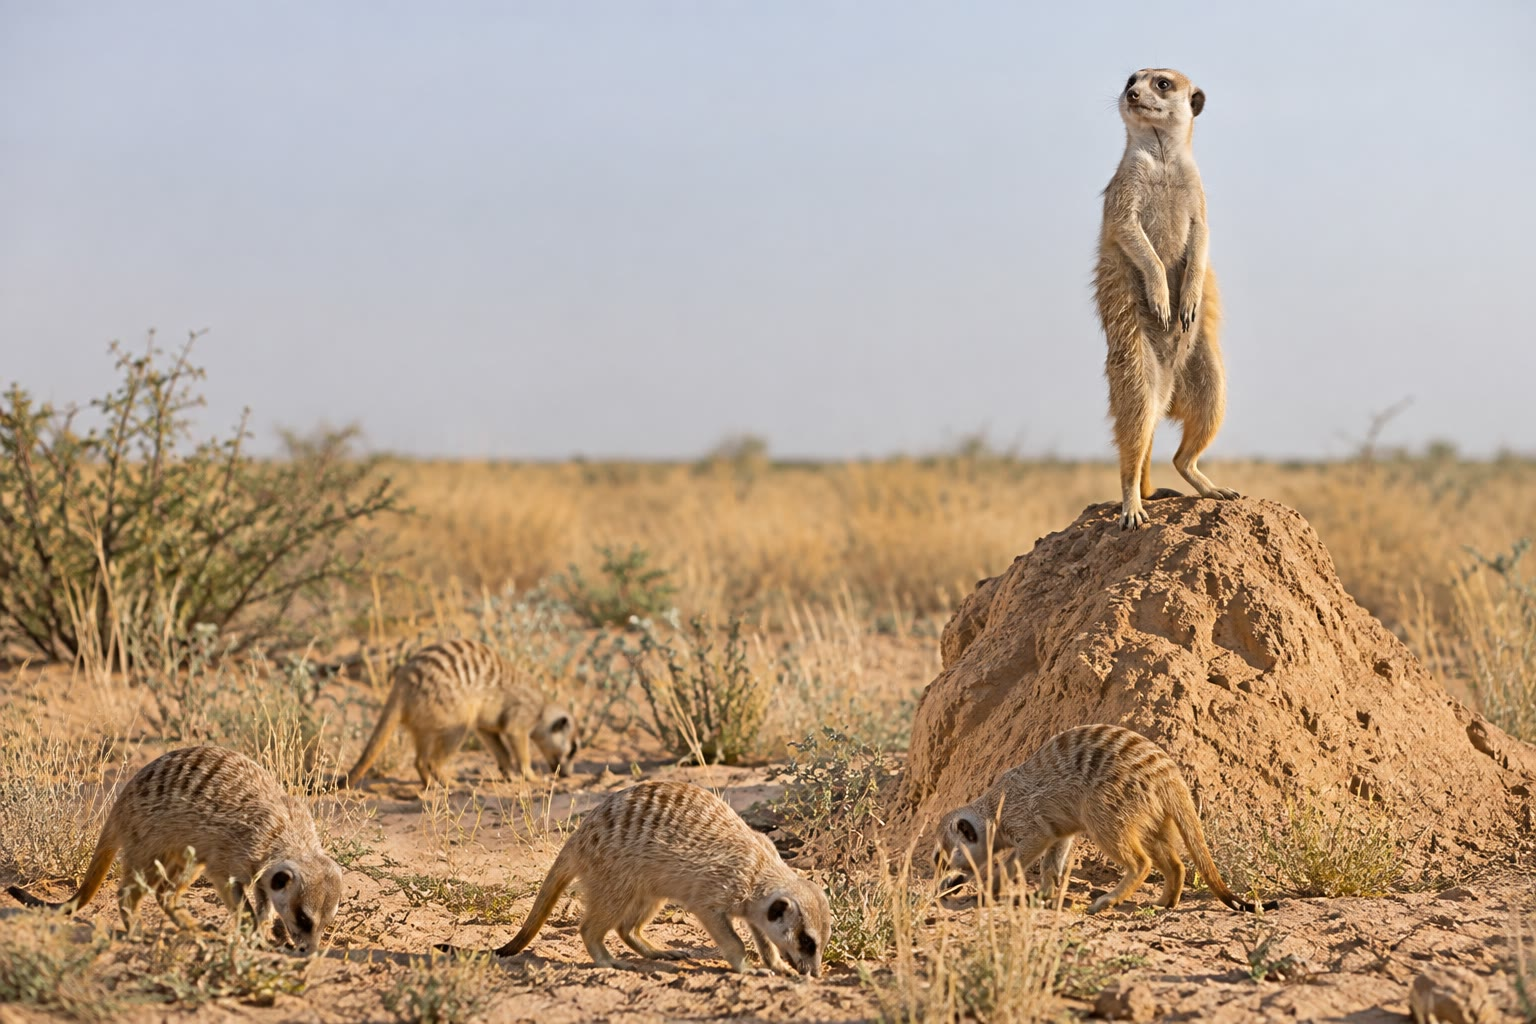
\includegraphics[width=0.46\linewidth]{images/book5/ai/b5-26-meerkat-sentinel.jpg}\hspace{0.04\linewidth}
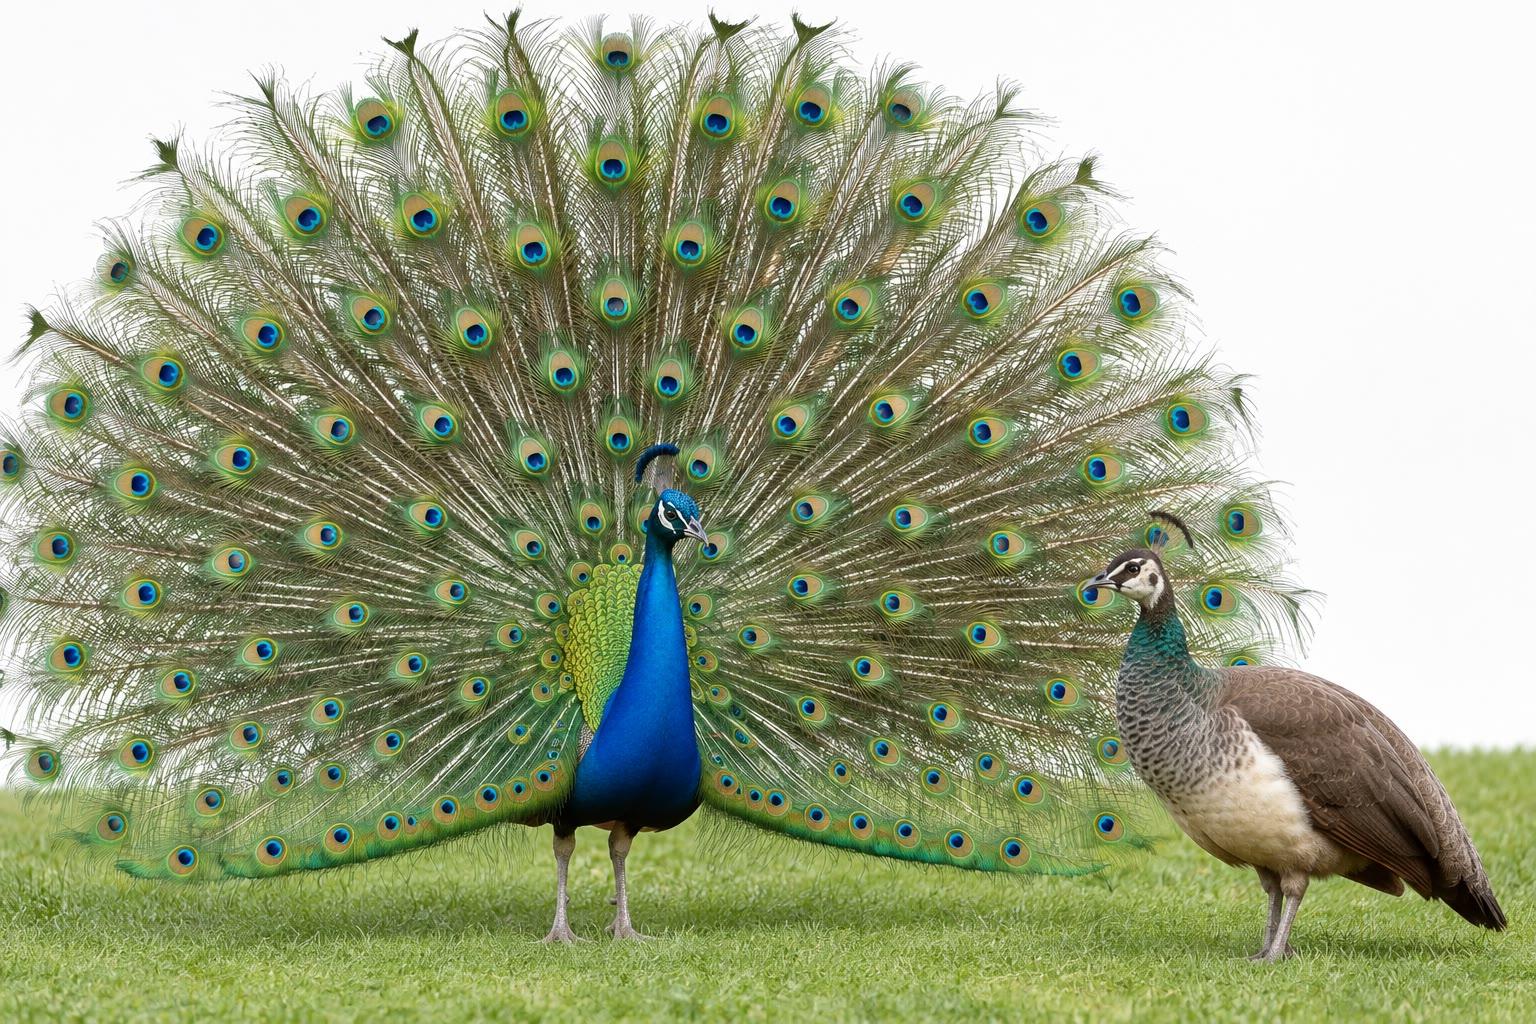
\includegraphics[width=0.46\linewidth]{images/book5/ai/b5-26-peacock-display.jpg}

{\small Links: een stokstaartje op schildwacht boven een foeragerende
groep van zijn verwanten. Rechts: een pauw die voor een pauwin pronkt
--- een bouwsel dat zijn drager voedsel en snelheid kost en hem niets
anders oplevert dan haar aandacht.}
\end{omfigure}

\section{Partners en boodschappen}

\begin{definition}[Seksuele selectie]\label{def:b3:behavioural-ecology:sexual-selection}
\index{seksuele selectie}\index{gradiënt van Bateman}\index{op hol geslagen selectie}\index{handicapbeginsel}\index{goede genen}\index{seksueel conflict}
Het tweede mechanisme van Darwin: selectie op kenmerken die partners
winnen in plaats van overleving. Haar wortel is de anisogamie --- de
voortplanting van een vrouwtje wordt begrensd door de eieren die zij
kan maken en voorzien, die van een mannetje door de vrouwtjes die hij
kan bevruchten --- zodat bij de meeste soorten de fitness van een
mannetje steil stijgt met zijn aantal paringen en die van een vrouwtje
nauwelijks (de \emph{gradiënt van Bateman}); mannetjes wedijveren dan
om vrouwtjes en vrouwtjes kiezen onder de mannetjes. De wedijver geeft
horens, geweien, slagtanden, een grote gestalte en de wedstrijden van
de vorige paragraaf. De keuze geeft sieraden, en drie verklaringen
waarom vrouwtjes daaraan de voorkeur geven. De \emph{op hol geslagen}
selectie van Fisher: een voorkeur voor een iets langere staart en de
langere staart verspreidden zich samen, waarbij elk de ander voordelig
maakte, tot de overlevingskosten van de staart zijn winst aan paringen
in evenwicht hielden. De \emph{handicap} van Zahavi: een sieraad dat
alleen een gezond mannetje zich kan veroorloven te laten groeien is een
\omterm{prop:b3:behavioural-ecology:signals}{eerlijk signaal} van zijn conditie, juist omdat het duur is --- een pauw
met een volle sleep heeft aantoonbaar minder parasieten. \emph{Goede
genen} en \emph{rechtstreekse voordelen}: het vrouwtje wint, door wat
haar nakomelingen erven of door het territorium en het voedsel dat het
mannetje levert. De belangen van de twee geslachten lopen uiteen, en
het \emph{seksuele conflict} --- over de paarfrequentie, over wie er
voor de jongen zorgt, over het lot van het zaad van een vorige partner
--- is een wapenwedloop binnen één soort: het zaadvocht van mannelijke
fruitvliegen verkort het leven van het vrouwtje en verhoogt haar
eileg, en vrouwtjes ontwikkelen weerstand.
\end{definition}

\begin{proof}[Bewijsmateriaal]
Andersson (1982) knipte en lijmde de staartveren van mannelijke
langstaartwidavogels in Kenia: mannetjes wier staart tot het dubbele
van de natuurlijke lengte was verlengd trokken vier maal zoveel nieuwe
nesten naar hun territorium als mannetjes met ingekorte staarten,
terwijl de controles wier staart werd afgeknipt en onveranderd
teruggelijmd niet werden beïnvloed --- de vrouwtjes hadden een voorkeur
voor een langere staart dan enig mannetje laat groeien, het kenmerk van
een voorkeur die verder is geselecteerd dan het kenmerk zelf. Petrie
(1994) vond dat pauwinnen paarden met de mannetjes wier sleep de meeste
ogen droeg, en dat de kuikens van die mannetjes het beter deden in de
bossen waar zij werden uitgezet --- een voordeel van \omterm{def:b3:behavioural-ecology:sexual-selection}{goede genen}
gemeten. Bateman (1948) telde de paringen en de nakomelingen van
fruitvliegen die merkermutaties droegen en vond de gradiënt die zijn
naam draagt: het voortplantingssucces van de mannetjes steeg lineair
met het aantal paringen, dat van de vrouwtjes vlakte na één paring af.
\end{proof}

\begin{proposition}[Eerlijke signalen]\label{prop:b3:behavioural-ecology:signals}
\index{communicatie}\index{eerlijk signaal}\index{kwispeldans}\index{verwijzend signaal}
Een signaal is een handeling die het gedrag van een ontvanger verandert
en die daartoe is geëvolueerd; het is alleen stabiel als het gemiddeld
voor beide partijen loont om het te zenden en erop te antwoorden. Waar
de twee gemeenschappelijke belangen hebben kan het signaal goedkoop en
nauwkeurig zijn: de \emph{kwispeldans} van een foeragerende honingbij
(von Frisch, jaren 1940) codeert de richting van een voedselbron als de
hoek van de kwispelloop met de verticaal --- de hoek van de bron met de
zon --- en de afstand als de duur van de loop, ongeveer een seconde per
kilometer, en de gerekruteerde bijen vliegen tot op enkele tientallen
meters van het doel; meerkatten geven verschillende alarmroepen voor
luipaarden, arenden en slangen, en luisteraars antwoorden passend op
elke roep die uit een verborgen luidspreker klinkt ---
\emph{verwijzende} signalen. Waar de belangen botsen moet een signaal
duur of niet na te maken zijn om eerlijk te blijven --- het burlen van
een mannelijk edelhert, wier tempo alleen een fit hert kan volhouden;
de grootte van de kwaak van een pad, bepaald door zijn lichaam; de
sieraden van de vorige alinea --- of het wordt uitgebuit: vuurvliegjes
van het ene geslacht bootsen de flitsen van de vrouwtjes van een ander
na om de mannetjes op te eten die erop afkomen, en de bedelroep van een
koekoeksjong overtroeft die van de eigen jongen van de gastheer. De
theorie van het signaleren voorspelt dus de vorm van een signaal uit de
verhouding tussen de partijen: goedkoop en informatief tussen verwanten
en partners wier belangen samenvallen, duur en geritualiseerd tussen
rivalen, en een wapenwedloop tussen roofdier en prooi.
\end{proposition}
\admitted

\begin{omfigure}
\begin{tikzpicture}[every node/.style={font=\scriptsize}, >=stealth]
  % field view
  \node[above] at (0,3.2) {in het veld};
  \draw[->, thick, gray] (0,0) -- (0,2.6) node[above, font=\tiny] {naar de zon};
  \fill[omDef!60] (0,0) circle (0.12); \node[below, font=\tiny] at (0,-0.2) {bijenkast};
  \draw[->, very thick, omThm] (0,0) -- ({2.4*sin(40)},{2.4*cos(40)}); \node[right, font=\tiny, omThm] at ({2.4*sin(40)},{2.4*cos(40)}) {voedsel, \qty{1}{km}};
  \draw[omThm] (0,1.0) arc[start angle=90, end angle=50, radius=1.0]; \node[font=\tiny, omThm] at (0.55,1.25) {$40^{\circ}$};
  % comb view
  \begin{scope}[shift={(6.2,0)}]
    \node[above] at (0,3.2) {op de verticale raat};
    \draw[very thick, gray!60] (-1.8,-0.4) rectangle (1.8,3.0);
    \draw[->, thick, gray] (0,0) -- (0,2.6) node[above, font=\tiny] {omhoog (= zon)};
    \draw[->, very thick, omThm] (0,0) -- ({1.6*sin(40)},{1.6*cos(40)}); \node[below, align=center, font=\tiny, omThm] at (0,-0.5) {kwispelloop: $40^{\circ}$ van de verticaal;\\duur $\approx \qty{1}{s}$ per km};
    \draw[omThm, dashed] ({1.6*sin(40)},{1.6*cos(40)}) .. controls (1.3,0.4) and (0.5,-0.3) .. (0,0);
    \draw[omThm, dashed] ({1.6*sin(40)},{1.6*cos(40)}) .. controls (-0.2,1.2) and (-0.6,0.3) .. (0,0);
    \draw[omThm] (0,0.8) arc[start angle=90, end angle=50, radius=0.8]; \node[font=\tiny, omThm] at (0.45,1.0) {$40^{\circ}$};
  \end{scope}
  \node[right, align=left] at (9.2,1.3) {een symbolische code: de zwaartekracht\\staat voor de zon, de tijd\\voor de afstand; de gerekruteerde bijen\\komen op tientallen meters aan};
\end{tikzpicture}

{\small De kwispeldans. De hoek van de loop met de verticaal is de hoek
van het voedsel met de zon; de lengte van de loop is de afstand. Een
signaal dat zo goedkoop en zo nauwkeurig is kan bestaan omdat de
danseres en haar publiek zussen met hetzelfde belang zijn.}
\end{omfigure}

\begin{omfigure}
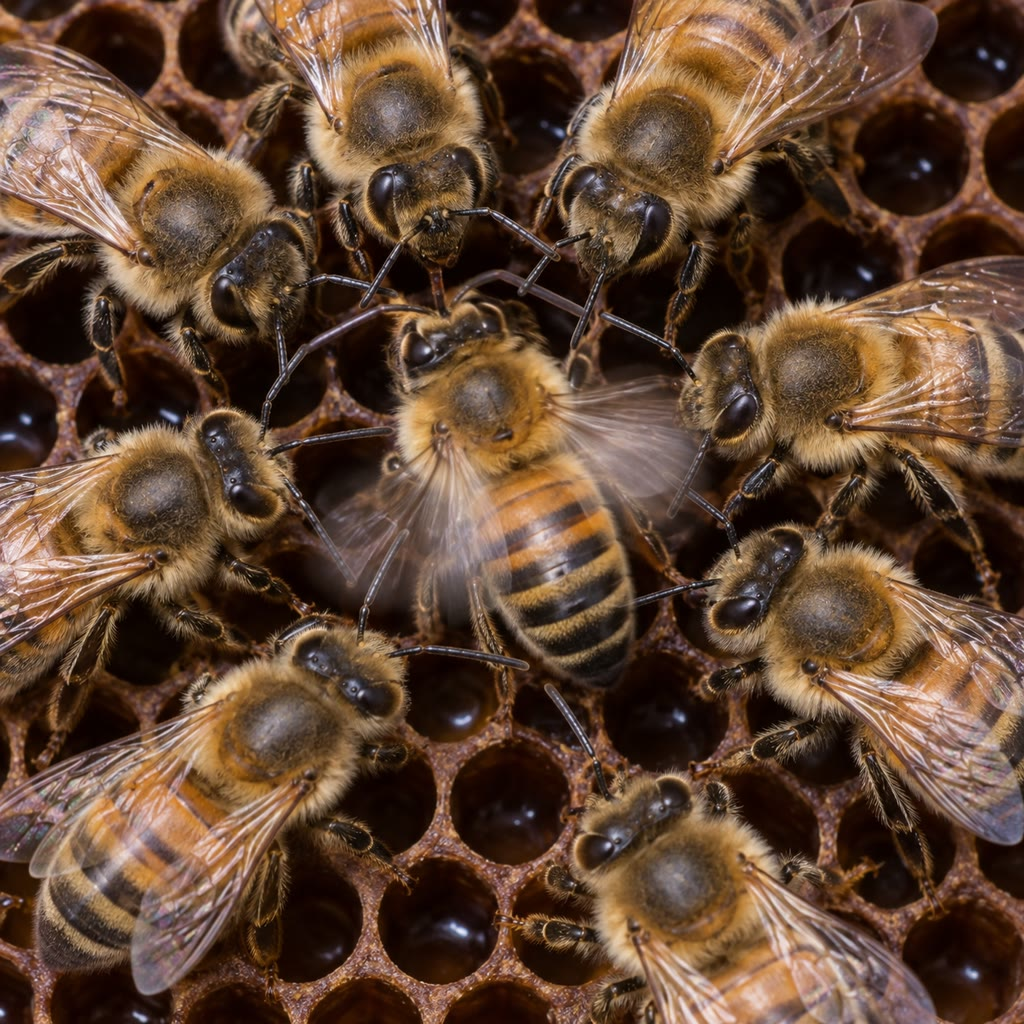
\includegraphics[width=0.4\linewidth]{images/book5/ai/b5-26-bee-dance.jpg}

{\small Een foerageerster die op de raat danst, omringd door werksters
die de hoek en het tempo van haar loop aflezen.}
\end{omfigure}

\begin{remark}[Waarom dieren lijken te rekenen]\label{rem:b3:behavioural-ecology:remark}
De koolmees differentieert $g(t)/(\tau + t)$ niet, het stokstaartje
berekent $r$ niet, en de pauwin heeft nooit van een handicap gehoord.
Elk draagt regels --- vertrek wanneer de vangsten trager worden, roep
wanneer de groep familie is, kies de helderste --- die de selectie
heeft gevormd omdat dieren die ze volgden meer nakomelingen
achterlieten; de wiskunde is van ons, een manier om te vragen wat de
regels moeten bereiken opdat dat zo is, en om gedrag te voorspellen in
situaties die de dieren nooit hebben meegemaakt. Wanneer de
voorspellingen falen --- de mees blijft te lang, de kosten van de
schildwacht vallen lager uit dan verondersteld --- is dat falen
leerzaam: een valuta was verkeerd, een beperking werd over het hoofd
gezien, een verwant werd verkeerd geteld. Het vak is een gesprek van
decennium tot decennium tussen een veldnotitieboek en een regel
algebra, en de vier vragen die Tinbergen stelde blijven het kader voor
beide.
\end{remark}

\section{Opgaven}

\begin{exercise}[$\star$]\label{exo:b3:behavioural-ecology:1}
Formuleer de \omterm{def:b3:behavioural-ecology:tinbergen}{vier vragen van Tinbergen} en beantwoord ze elk, in één
zin, voor de kwispeldans.
\end{exercise}

\begin{exercise}[$\star$]\label{exo:b3:behavioural-ecology:2}
Wat is een \omterm{def:b3:behavioural-ecology:tinbergen}{vast handelingspatroon} en wat een \omterm{def:b3:behavioural-ecology:tinbergen}{sleutelprikkel}? Geef twee
voorbeelden en leg uit wat het ``bovennormale'' stokje met drie rode
banden liet zien.
\end{exercise}

\begin{exercise}[$\star$]\label{exo:b3:behavioural-ecology:3}
Wat zegt de \omterm{thm:b3:behavioural-ecology:mvt}{stelling van de marginale waarde}, in woorden, en wat
voorspelt zij over het gebruik van plekken wanneer de reistijd
verdubbelt?
\end{exercise}

\begin{exercise}[$\star$]\label{exo:b3:behavioural-ecology:4}
Definieer een ESS. Waarom is een populatie van louter Duiven er geen,
en waarom kost het mengsel Havik--Duif iedereen iets?
\end{exercise}

\begin{exercise}[$\star\star$]\label{exo:b3:behavioural-ecology:5}
Havik--Duif met $V = 6$, $C = 10$: bereken $p^{*}$, de opbrengst van
elke strategie bij de ESS, en de opbrengst die een populatie van louter
Duiven zou hebben. Herhaal voor $V = 12$, $C = 10$.
\end{exercise}

\begin{exercise}[$\star\star$]\label{exo:b3:behavioural-ecology:6}
Een winstfunctie $g(t) = A(1 - \mathrm{e}^{-t/T_{0}})$ met $T_{0} =
\qty{2}{min}$. Bepaal $t^{*}$ voor $\tau = 2$ en $\tau = 8$ minuten
(gebruik de waarden uit het hoofdstuk), het deel van elke plek dat
wordt opgegeten, en het tempo $R$ op den duur als fractie van $A$ per
minuut.
\end{exercise}

\begin{exercise}[$\star\star$]\label{exo:b3:behavioural-ecology:7}
Bereken $r$ tussen: halfbroers en halfzussen; grootouder en kleinkind;
volle neven en nichten; een haplodiploïde werkster en haar broer; een
haplodiploïde koningin en haar zoon. Verklaar de laatste twee.
\end{exercise}

\begin{exercise}[$\star\star$]\label{exo:b3:behavioural-ecology:8}
Een alarmroep kost de roeper een kans van \qty{2}{\%} om te sterven en
behoedt elk van $n$ nabije verwanten voor een kans van \qty{1}{\%}.
Voor welke $n$ pleit de \omterm{thm:b3:behavioural-ecology:hamilton}{regel van Hamilton} voor roepen als de verwanten
volle broers en zussen zijn? En als het nichtjes zijn? En als zij niet
verwant zijn?
\end{exercise}

\begin{exercise}[$\star\star$]\label{exo:b3:behavioural-ecology:9}
De staart van een widavogel is \qty{50}{cm}; tot \qty{75}{cm} verlengd
trekt hij tweemaal zoveel nesten, tot \qty{25}{cm} ingekort de helft.
Als de overleving met \qty{20}{\%} daalt voor elke \qty{25}{cm} die
erbij komt, welke staart maximaliseert dan het product van paringen en
overleving, en waarom zou de natuurlijke staart korter kunnen zijn?
\end{exercise}

\begin{exercise}[$\star\star\star$]\label{exo:b3:behavioural-ecology:10}
Voeg een derde strategie toe, Vergelder, die vertoont als een Duif maar
terugvecht wanneer zij wordt aangevallen. Schrijf haar opbrengsten
tegen Havik, Duif en zichzelf op (tegen Havik vecht zij: $(V - C)/2$;
tegen Duif en Vergelder deelt zij: $V/2$). Laat zien dat een populatie
Vergelders niet door Haviken kan worden binnengedrongen wanneer $V < C$,
en bespreek of Duiven er binnen kunnen drijven.
\end{exercise}

\begin{exercise}[$\star\star\star$]\label{exo:b3:behavioural-ecology:11}
Bij een uitputtingsslag houdt elke deelnemer het vol gedurende een tijd
uit een verdeling; de ESS is exponentieel met gemiddelde $V/$(kosten
per tijdseenheid). Leg uit waarom een vaste volhoudtijd geen ESS kan
zijn, en waarom een exponentiële verdeling het verwachte verdere
volhouden van een tegenstander die nog vertoont onafhankelijk maakt van
hoe lang hij dat al doet.
\end{exercise}

\begin{exercise}[$\star\star\star$]\label{exo:b3:behavioural-ecology:12}
Het betoog van Hamilton over de haplodiploïdie voorspelt dat werksters
liever zussen ($r = 3/4$) dan broers ($r = 1/4$) grootbrengen, terwijl
de koningin zonen en dochters even hoog waardeert. Voorspel de
geslachtsverhouding van de voortplantende dieren die een kolonie zou
moeten voortbrengen als de werksters die bepalen, en als de koningin
dat doet; zeg wat Trivers en Hare vonden, en wat een koningin die met
verscheidene mannetjes paart met het betoog doet.
\end{exercise}

\section{Vraagstuk: de rekensom van de schildwacht}

\begin{problem}[{Weekendvraagstuk --- een dag in een groep
stokstaartjes als gedragsecologie gedaan: de verblijftijden van de
stelling van de marginale waarde, de wedstrijden van het spel
Havik--Duif en de ESS ervan, de verwantschapsboekhouding van de
schildwachtdienst en van een haplodiploïd bijenvolk, en de kosten van
een sieraad, eindigend bij de verblijftijd in een plek, de frequentie
van de Haviken en de drempel van Hamilton voor de schildwacht}]
\label{pb:b3:behavioural-ecology:1}
Gegevens: foerageerplekken met $g(t) = A(1 - \mathrm{e}^{-t/T_{0}})$, $T_{0}
= \qty{3}{min}$, $A = \qty{60}{kJ}$; reis tussen de plekken $\tau =
\qty{3}{min}$ (dicht leefgebied) of \qty{12}{min} (ijl). Wedstrijden om
een hol: $V = 10$, $C = 30$ (fitnesseenheden). Schildwacht: een uur
dienst kost de schildwacht $c = 0.03$ nakomelingequivalenten (gemist
voedsel, blootstelling); het verlaagt het roofdierrisico van elk
groepslid, elk $b = 0.01$ nakomelingequivalent waard; de groep telt $n$
leden met een gemiddelde verwantschap $\bar r$. Bijenvolk: een werkster
kan met dezelfde inspanning ofwel $k$ zussen ofwel $k$ eigen dochters
grootbrengen. Sieraad: staartlengte $L$ geeft paringen $m(L) = L/20$ en
overleving $s(L) = 1 - (L/100)^{2}$, met $L$ in cm.

\medskip
\noindent\textbf{Deel I --- Plekken.}
\begin{enumerate}
  \item Schrijf het tempo $R(t)$ op den duur op en de voorwaarde van de
        marginale waarde voor deze $g$.
  \item Laat zien dat de voorwaarde herleidt tot $(\tau + t)/T_{0} = \mathrm{e}^{t/T_{0}}
        - 1$, en los haar op voor $\tau = T_{0}$ (probeer $t = 1.15\,T_{0}$).
  \item Los op voor $\tau = 4T_{0}$ (probeer $t = 2.0\,T_{0}$).
  \item Voor elk geval: de verblijftijd in minuten, de energie per plek,
        het deel van de plek dat wordt opgegeten, en het tempo $R$ in kJ/min.
  \item Een vuistregel: ``vertrek na een vaste \qty{5}{min}''. Bereken
        $R$ voor beide leefgebieden en vergelijk met het optimum. Is de
        regel goed genoeg?
  \item Een andere regel: ``vertrek wanneer er \qty{20}{s} voorbijgaan
        zonder vangst''. Leg uit waarom deze regel van de opgeeftijd de
        stelling benadert, en in welke richting zij faalt wanneer
        plekken in rijkdom verschillen.
\end{enumerate}

\medskip
\noindent\textbf{Deel II --- Wedstrijden.}
\begin{enumerate}[resume]
  \item Schrijf de opbrengstmatrix op en bereken $p^{*}$.
  \item De opbrengst van Havik en van Duif bij $p = 0.1$, $p = p^{*}$ en $p =
        0.6$; welke strategie breidt zich in elk geval uit?
  \item De opbrengst bij de ESS; vergelijk met de opbrengst bij louter
        Duiven. Hoeveel verliest de populatie per wedstrijd aan de
        mogelijkheid van vechten?
  \item Een droogte verhoogt $V$ tot $40$ (holen worden schaars). Nieuwe
        ESS? Wat voorspelt dat over gevechten in zware jaren?
  \item Bourgeois: ``Havik als bewoner, Duif als indringer'', met elke
        rol de helft van de tijd. Haar opbrengst tegen zichzelf is $V/2$
        zonder gevechten. Laat zien dat Haviken een populatie Bourgeois
        niet kunnen binnendringen wanneer $V
        < C$, en verklaar het bont zandoogje.
  \item Leg in één zin uit waarom hier de frequentieafhankelijkheid en
        niet een optimum dit gedrag bestuurt.
\end{enumerate}

\medskip
\noindent\textbf{Deel III --- Verwanten.}
\begin{enumerate}[resume]
  \item De \omterm{thm:b3:behavioural-ecology:hamilton}{regel van Hamilton} voor de schildwacht: de voorwaarde op
        $n\bar r$. Voor welke $n\bar r$ loont de dienst?
  \item Een groep van $n = 8$ volle broers en zussen ($\bar r = 1/2$):
        loont het? Een groep van 8 niet-verwante dieren? Een groep van 8
        halfbroers en halfzussen?
  \item De schildwacht is goed gevoed, zodat zijn $c$ tot $0.01$ daalt.
        Wat is de drempel nu? Waarom voorspelt dat dat de schildwachten
        de goed gevoede dieren zijn?
  \item Het bijenvolk: de waarde in \omterm{thm:b3:behavioural-ecology:hamilton}{inclusieve fitness} van $k$ zussen
        tegen $k$ dochters. Wat zou een werkster moeten verkiezen, en
        met welke verhouding?
  \item De koningin heeft in gelijke mate met drie mannetjes gepaard:
        de gemiddelde verwantschap van de werksters met hun zussen?
        Blijft de voorkeur bestaan?
  \item Leg uit waarom de \omterm{thm:b3:behavioural-ecology:hamilton}{regel van Hamilton} niet vereist dat de
        handelende verwanten herkent, en welke vuistregel een
        grondeekhoorn in werkelijkheid zou kunnen gebruiken.
\end{enumerate}

\medskip
\noindent\textbf{Deel IV --- Sieraden.}
\begin{enumerate}[resume]
  \item Fitness $W(L) = m(L)\,s(L)$. Bereken $W$ voor $L = 20$, $40$, $60$
        en $80$.
  \item Bepaal analytisch de $L$ die $W$ maximaliseert, en $W$ daar.
  \item De overlevingskosten worden steiler, $s = 1 - (L/70)^{2}$ (er
        komt een roofdier bij). Nieuw optimum? In welke richting, en
        waarom voorspelt dit dat de staart in zijn evolutie de predatie
        volgt?
  \item Het experiment van Andersson verdubbelde de staarten tot
        \qty{75}{cm} en verdubbelde het aantal nesten. Is de voorkeur
        van de vrouwtjes voor langere staarten ``voorbij het optimum''
        in overeenstemming met de verklaring van de \omterm{def:b3:behavioural-ecology:sexual-selection}{op hol geslagen
        selectie}, met die van de handicap, of met beide?
  \item Waarom is een goedkoop sieraad geen \omterm{prop:b3:behavioural-ecology:signals}{eerlijk signaal}, en hoe
        maken de kosten uit vraag~21 het er wel een?
  \item Gradiënten van Bateman: mannetjes winnen $0.8$ nakomeling per
        extra paring, vrouwtjes $0.1$. Leg in één alinea uit hoe deze
        scheefheid zowel de wedstrijden van deel~II als de sieraden van
        deel~IV voortbrengt.
  \item Vat samen: $t^{*}$ in het dichte leefgebied (vraag~4), $p^{*}$
        (vraag~7), en de drempel $n\bar r$ van de schildwacht
        (vraag~13).
\end{enumerate}
\end{problem}
